\chapter{Manual de usuario}
\section{Objetivo}
El objetivo de este manual es proporcionar los pasos precisos para hacer uso del aplicativo web de Distrifull. 

\section{Vista principal}
Una vez que el usuario ingrese a la direcci\'on de la p\'agina web de Distrifull, observa la siguiente vista:
\begin{figure}[h!]
	\centering
	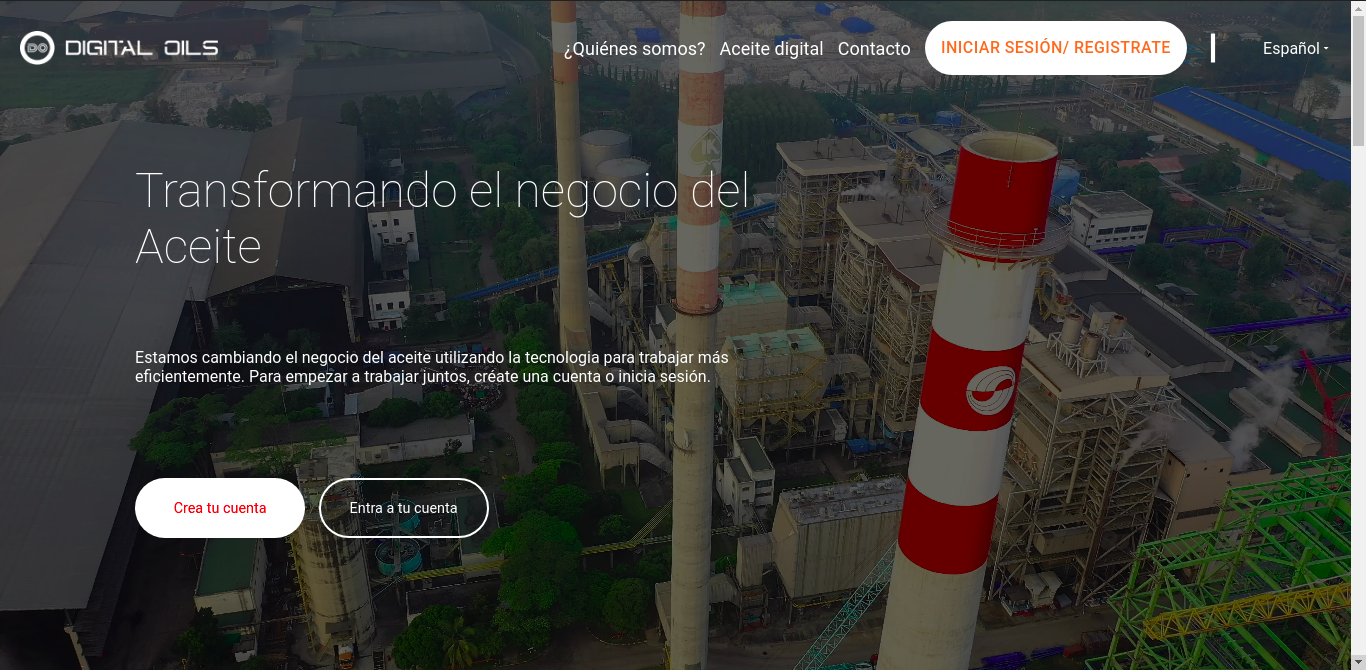
\includegraphics[width=0.9\linewidth, height=0.3\textheight]{imagenes/inicioOne}
	\caption[Primera parte del inicio.]{Vista principal}
	\label{fig:inicioone}
\end{figure}

Esta secci\'on encontramos en la parte superior izquierda el logo de la empresa y en la parte derecha encontramos acceso directo a las secciones visibles a todo tipo de usuario, entre ellas tenemos:
\begin{description}
	\item[ ?`Qui\'enes somos?: ] este bot\'on  nos lleva a la secci\'on donde encontramos una breve explicaci\'on sobre la empresa.
	\item[Aceite digital: ] este bot\'on nos lleva a una secci\'on donde encontramos productos de la empresa.
	\item[Iniciar sesi\'on y registrarse: ] este bot\'on nos lleva a la p\'agina de inicio de sesi\'on o la p\'agina de registro.
	\item[Idioma: ] en este bot\'on podemos cambiar el idioma, en este caso tenemos el espa\~nol y el ingl\'es. 
\end{description}
%\newpage
\subsection{Registro}
Para registrarnos en la p\'agina web desde la p\'agina principal mostrada en la figura \ref{fig:inicioone} presionamos el bot\'on registrarse y nos env\'ia a la siguiente p\'agina
\begin{figure}[h!]
	\centering
	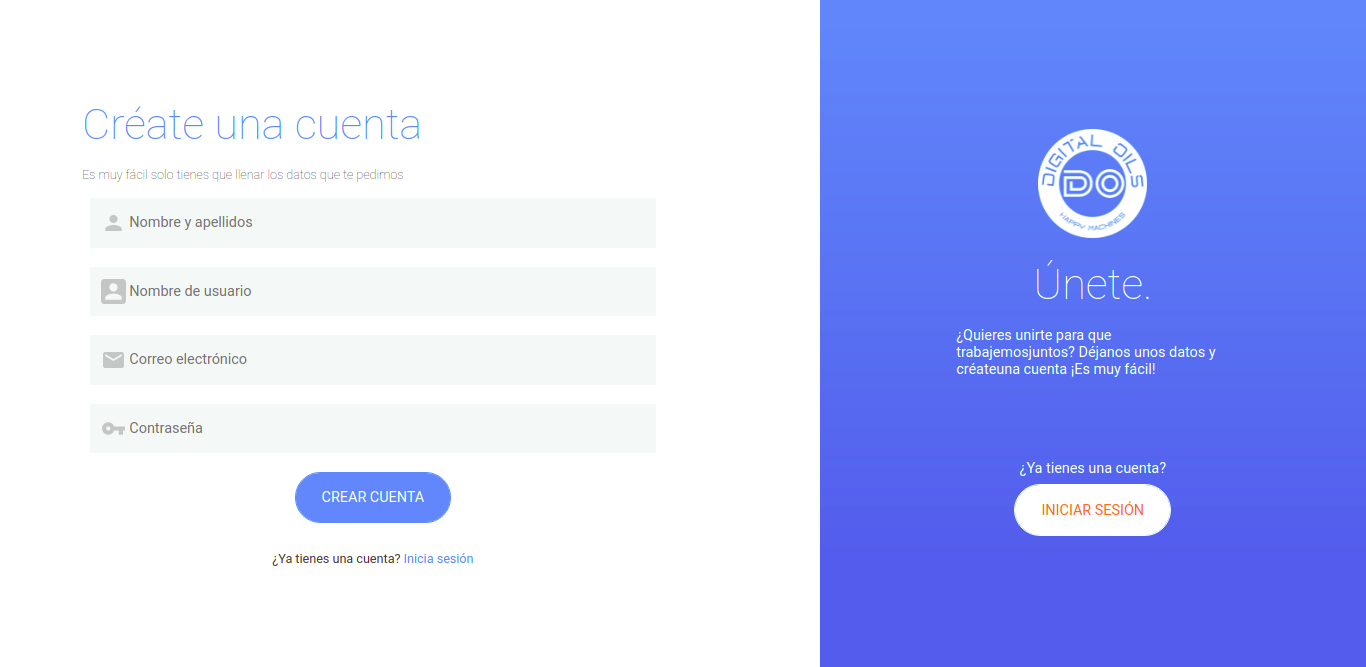
\includegraphics[width=1\linewidth, height=0.4\textheight]{imagenes/registro}
	\caption[Registro.]{Registro}
	\label{fig:inicioThree}
\end{figure}

Para realizar el registro en el aplicativo web, debemos llenar los siguientes campos: 
\begin{description}
	\item[Nombre y apellidos:] ingresar su nombre y apellidos para tener una experiencia personalizada en el sistema.
	\item[Nombre de usuario:] ingresar el nombre con que quiere ser identificado dentro de la plataforma.
	\item[Correo electr\'onico:] ingrese un correo electr\'onico al que tenga acceso, con este iniciara sesi\'on en la plataforma.
	\item[Contrase\~na:] elija una contrase\~na e ingr\'esela y tenga presente que debe recordarla para iniciar sesi\'on en la plataforma.
\end{description}
Una vez hemos culminado de llenar los campos, presionamos el bot\'on ``\textcolor{bluedistri}{CREAR CUENTA}'', apenas demos aceptar al mensaje de alerta, podemos presionar el bot\'on \textcolor{orangedistri}{iniciar sesi\'on} y accedemos a la parte interna de la p\'agina web.
\begin{figure}[h!]
	\centering
	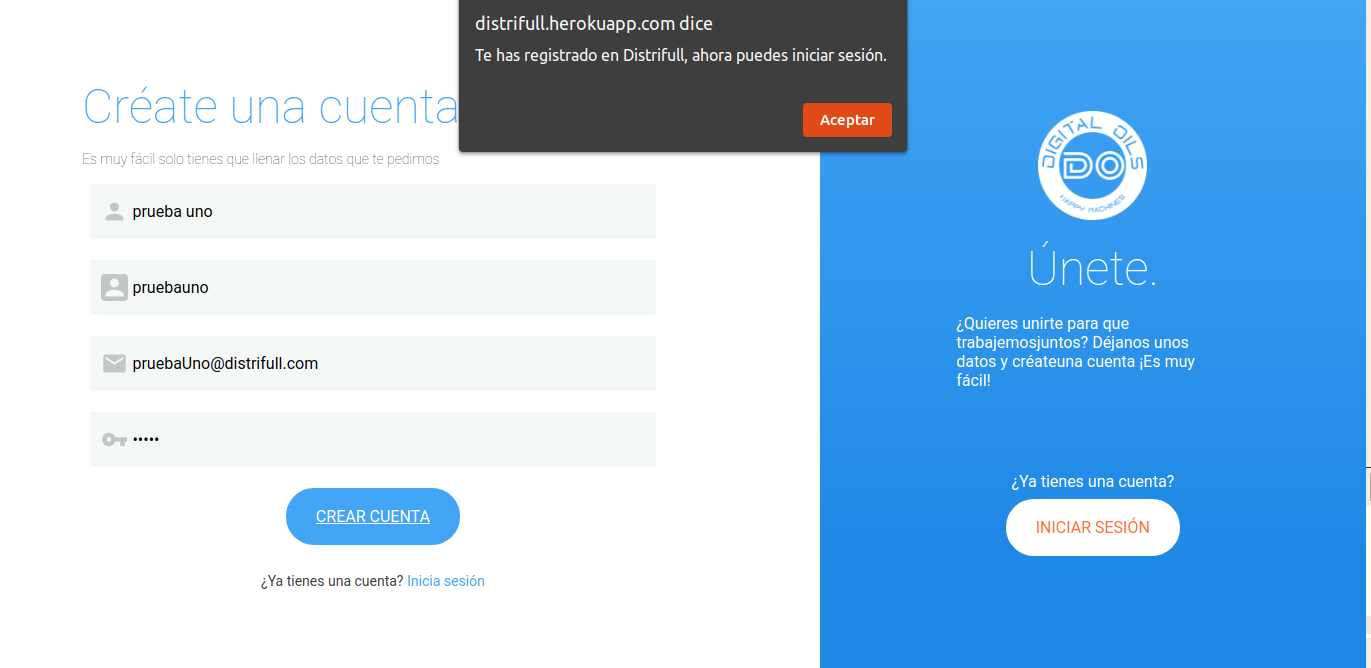
\includegraphics[width=1\linewidth, height=0.4\textheight]{imagenes/mensajeDeRegistro}
	\caption[Mensaje de registro.]{Mensaje de confirmaci\'on de registro.}
	\label{fig:mensajederegistro}
\end{figure}

\subsection{Inicio de sesi\'on}

\begin{figure}[h!]
	\centering
	\includegraphics[width=0.8\linewidth, height=0.2\textheight]{imagenes/inicioOneTE.png}
	\caption[Primera parte del inicio.]{Bot\'on p\'agina de inicio de sesi\'on}
	\label{fig:inicioonet}
\end{figure}
Al presionar el bot\'on \textcolor{orangedistri}{{\bf iniciar sesi\'on}}, nos env\'ia a la siguiente p\'agina:
\begin{figure}[h!]
	\centering
	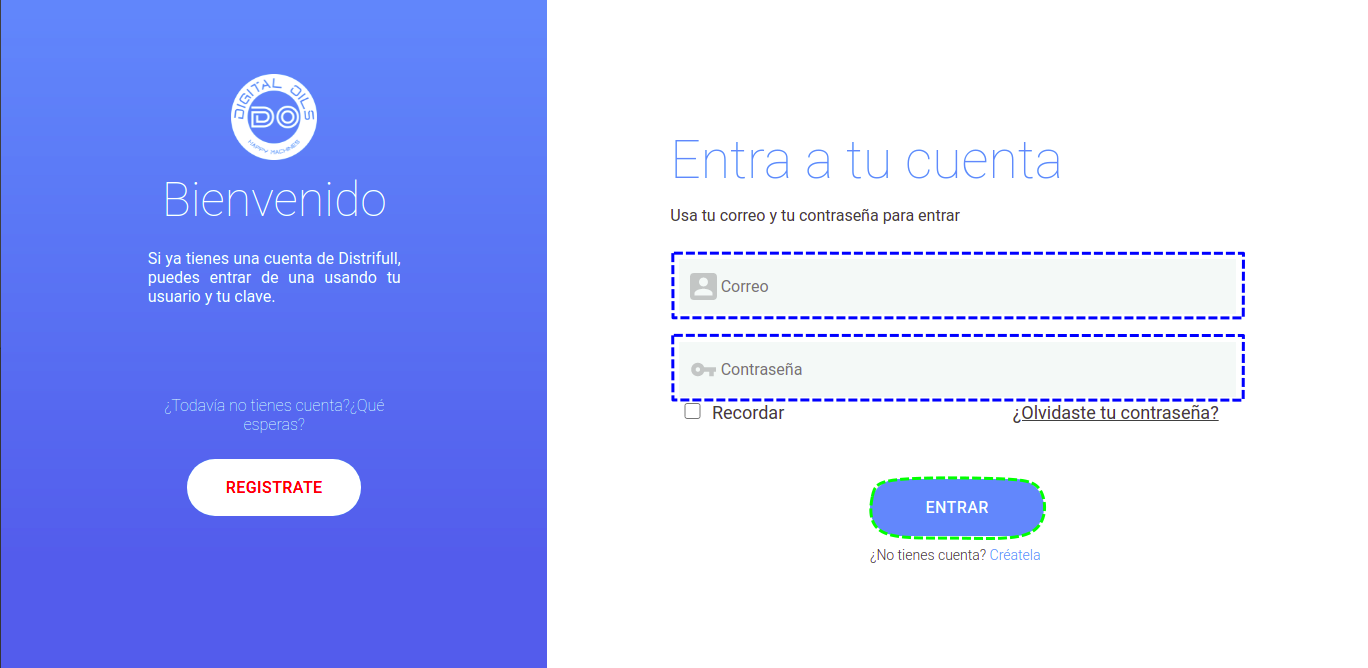
\includegraphics[width=0.9\linewidth, height=0.3\textheight]{imagenes/inicioSe}
	\caption[Inicio de sesi\'on.]{Inicio de sesi\'on.}
	\label{fig:iniciosesion}
\end{figure}
\newpage
Al ingresar los datos requeridos en cada campo, los cuales son: 
\begin{description}
	\item[Correo: ] En este campo ingresamos el correo con el cual hicimos el registro en la p\'agina Web.
	\item[Contrase\~na: ] En este campo ingresamos con la contrase\~na elegida al momento de realizar el registro en la plataforma.
\end{description}
Una vez tengamos todos los campos llenos, presionamos el bot\'on \textcolor{bluedistri}{{\bf\rm ENTRAR}}, si los datos son incorrectos el sistema no permite el ingreso y lanzara una alerta. Si son correctos, la 
vista que aparecer\'a depender\'a del tipo de usuario que seas, en este caso existen dos tipos de usuarios, el administrador y el no administrador.

Vista como administrador figura \ref{fig:dashboardInicio}: 


\begin{figure}[h!]
	\centering
	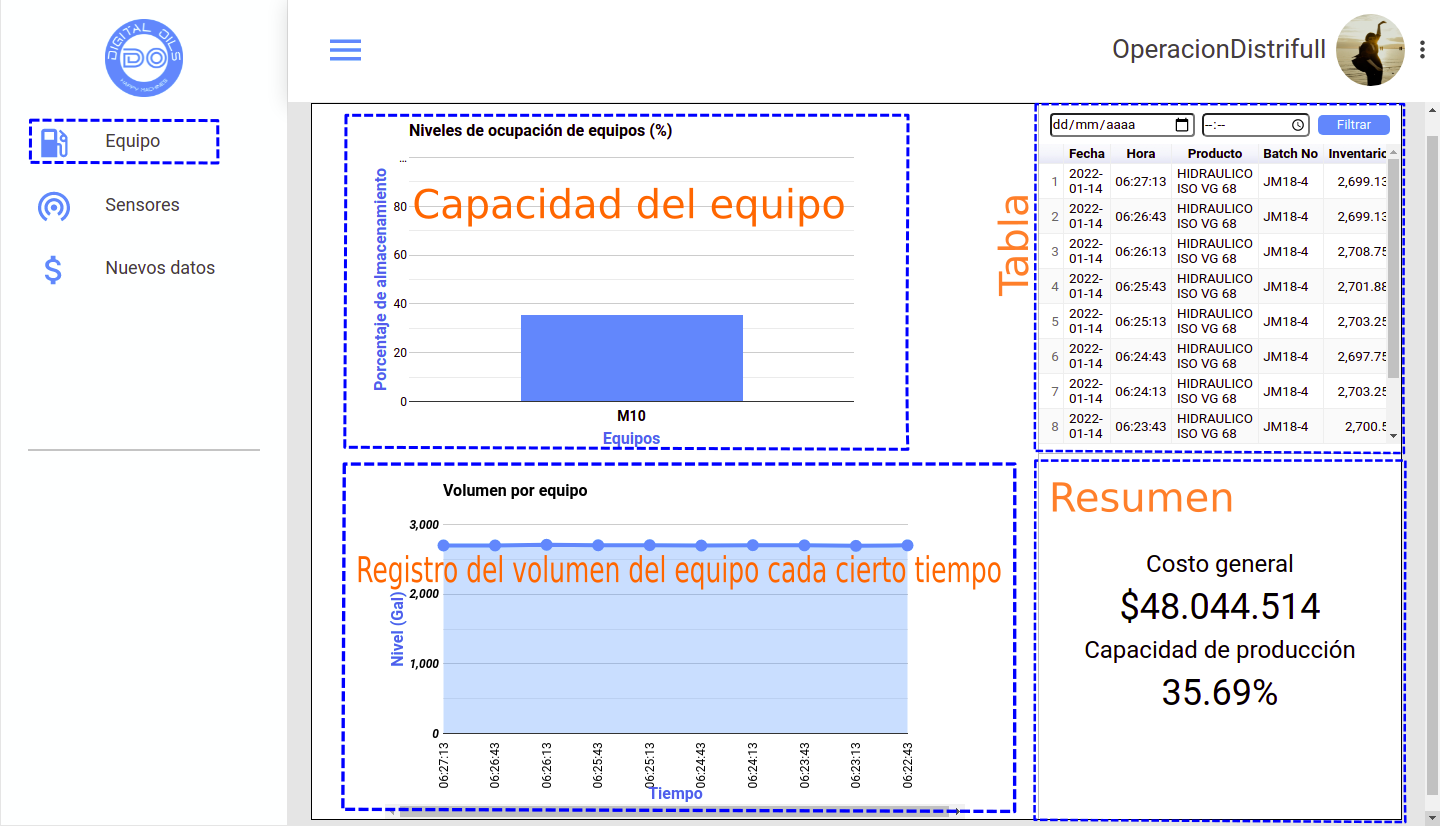
\includegraphics[width=1\linewidth, height=0.45\textheight]{imagenes/dashboardInicio}
	\caption[Dashboard equipo.]{Dashboard equipo}
	\label{fig:dashboardInicio}
\end{figure}

En la parte izquierda encontramos un men\'u deslizable, en la parte central encontramos la informaci\'on proporcionada por los sensores, la gr\'afica titulada {\bf Niveles de ocupaci\'on de equipos} proporciona informaci\'on sobre la capacidad del l\'iquido que tiene el tanque, la siguiente gr\'afica titulada {\bf Volumen por equipo} muestra la cantidad de l\'iquido que tiene el equipo por cierta cantidad de tiempo (cada 30 segundos), la tabla nos proporciona una parte de la informaci\'on captada por el sensor, que son fecha, hora producto, batch no (lote) y el inventario del tanque, finaliza con un \textcolor{orangedistri}{Resumen} que contiene el costo general y la capacidad de producci\'on del tanque.
\newpage
Vista sensores figura \ref{fig:dashboardSensores}: 
\begin{figure}[h!]
	\centering
	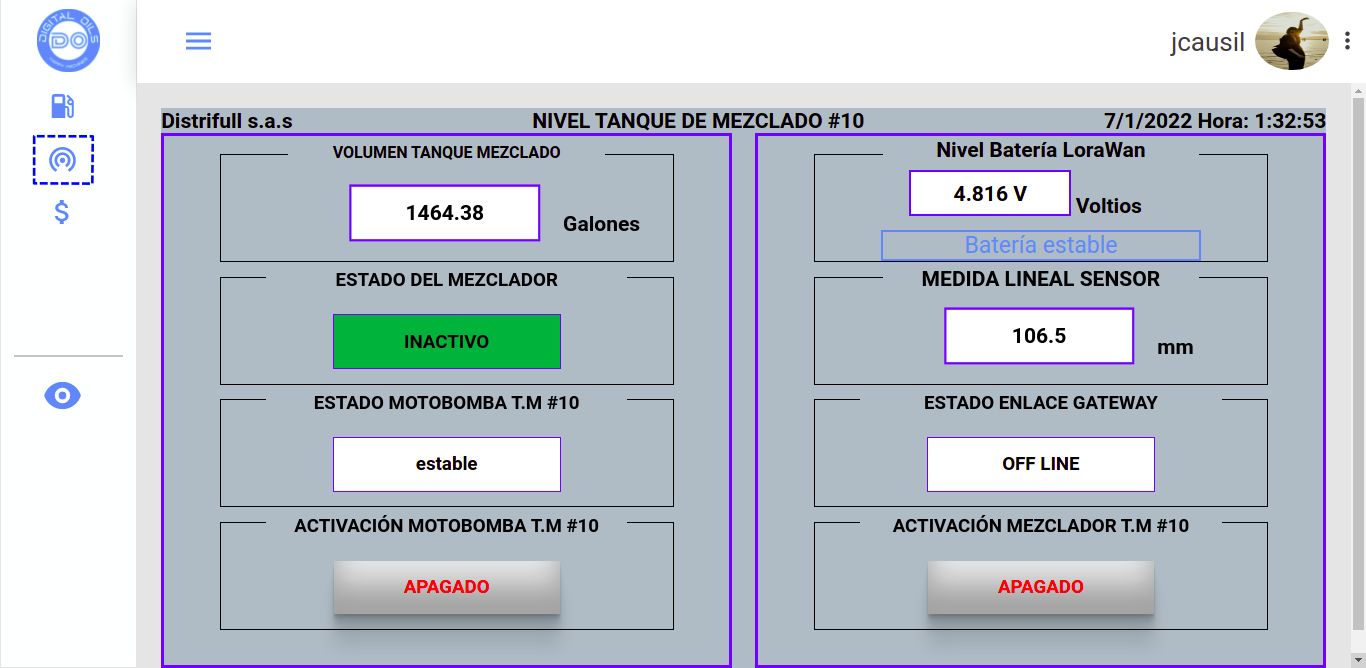
\includegraphics[width=1\linewidth, height=0.4\textheight]{imagenes/dashboardSensores}
	\caption[Dashboard sensores.]{Dashboard sensores}
	\label{fig:dashboardSensores}
\end{figure}

En esta p\'agina obtenemos: 
\begin{description}
	\item[Volumen tanque mezclado: ] indica la cantidad de producto en galones que tiene el equipo o tanque.
	\item[Estado del mezclador: ] indica si el l\'iquido est\'a en proceso de mezclado.
	\item[Estado motobomba: ] tiene tres estados, llenado nos indica que el tanque est\'a recibiendo producto, vaciado nos garantiza que el tanque est\'a evacuando producto y estable hace referencia a que se mantiene una misma cantidad de producto, es decir no sufre ning\'un cambio de volumen.
	\item[Activaci\'on motobomba: ] confirma si la moto bomba asociada al tanque est\'a encendida o apagada.
	\item[Nivel bater\'ia loraWan: ] este indicador nos permite darle seguimiento al estado de la bater\'ia, cuenta con dos estados ``Bater\'ia estable'' y ``Bater\'ia inestable''. 
	\item[Medida lineal sensor: ] indica la distancia entre el sensor y el producto en el tanque o equipo.
	\item[Activaci\'on mezclador: ] este indicador confirma si el producto o el l\'iquido en el equipo est\'a siendo mezclado, cuenta con dos estados ``APAGADO'' y ``ENCENDIDO''.
\end{description}
\newpage
Nuevos datos: 
\begin{figure}[h!]
	\centering
	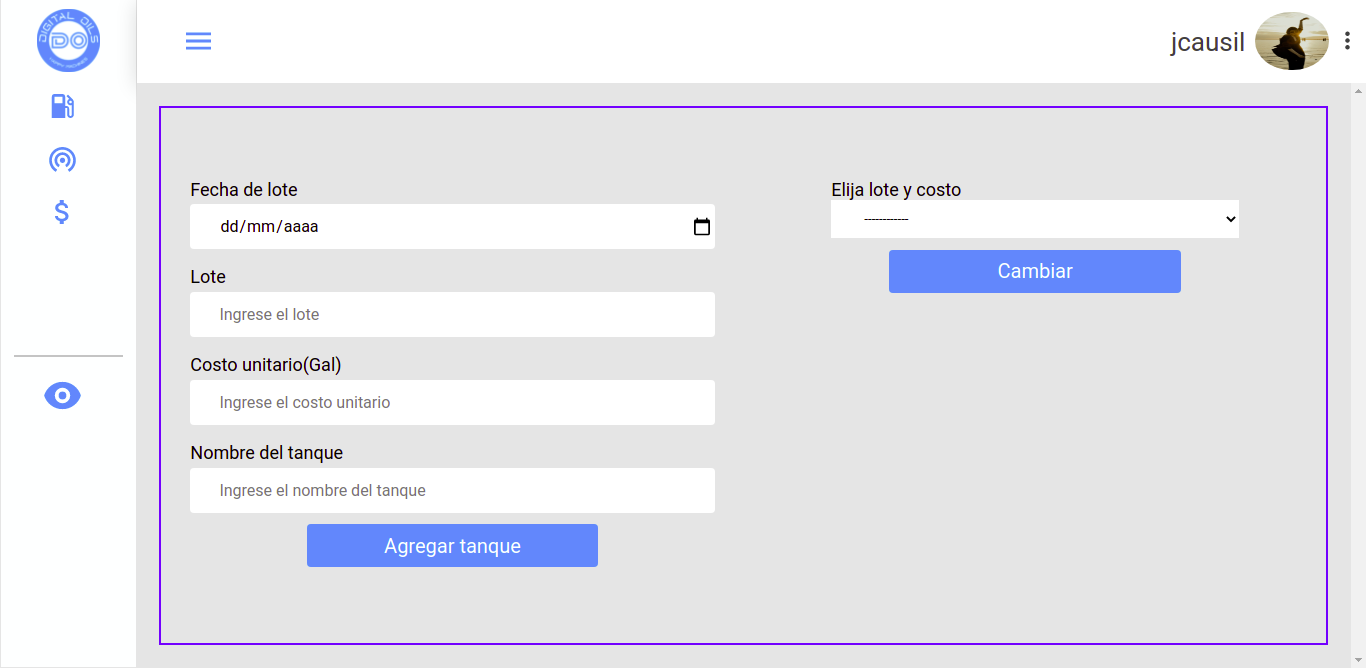
\includegraphics[width=1\linewidth, height=0.4\textheight]{imagenes/dashboardEstadistica}
	\caption[Dashboard nuevos datos.]{Dashboard nuevos datos}
	\label{fig:dashboardEstadistica}
\end{figure}

En esta vista podemos actualizar el costo por gal\'on y su respectivo lote, para hacer este cambio solo llenamos el formulario que tiene los siguientes campos: 
\begin{enumerate}[{\rm 1.}]
	\item Fecha de lote.
	\item Lote.
	\item Costo unitario.
	\item Nombre del tanque.
\end{enumerate}

Para finalizar el proceso presionamos el bot\'on ``\textcolor{bluedistri}{Agregar tanque}''.

En el campo ``Elija lote y costo'' tenemos un historial donde encontramos los diferentes costos que hemos ingresado, al presionar el bot\'on ``\textcolor{bluedistri}{Cambiar}'' se actualiza la informaci\'on de costo unitario, costo general y lote en la p\'agina equipos.
\newpage
{\bf Vista como no administrador}:

\begin{figure}[h!]
	\centering
	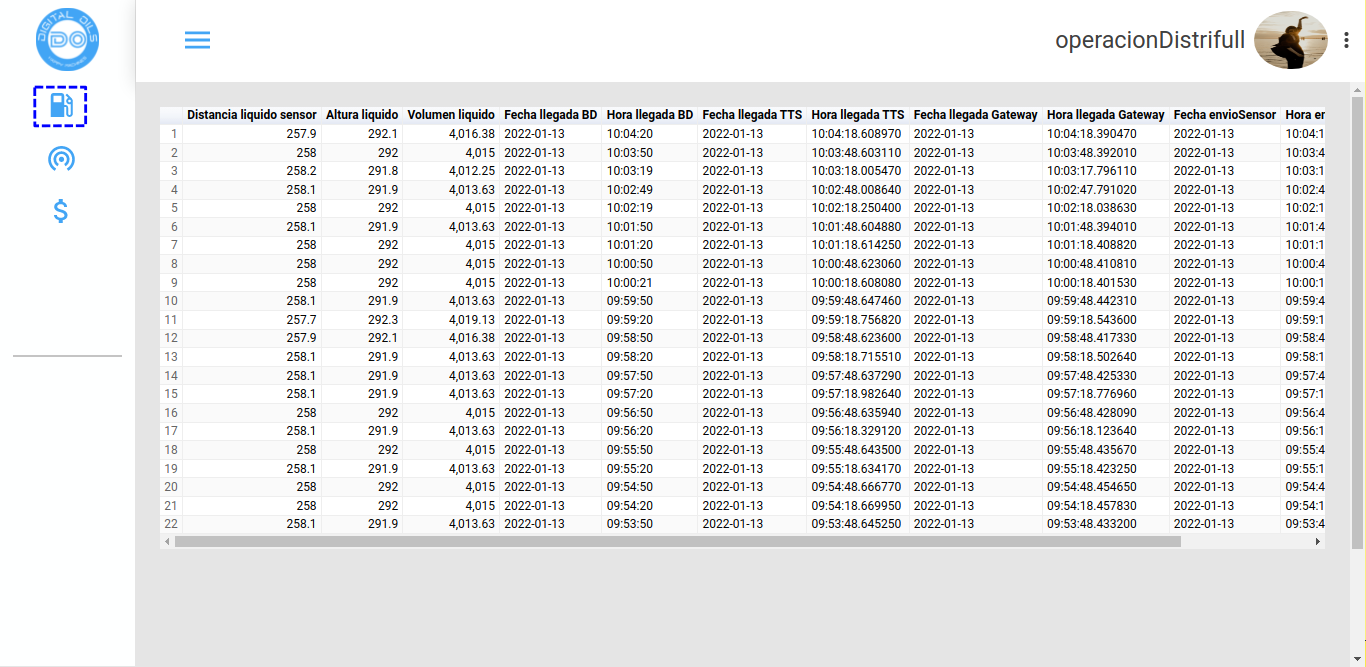
\includegraphics[width=1\linewidth, height=0.4\textheight]{imagenes/dashboardNoAdmi}
	\caption[Dashboard no admi.]{Dashboard no administrador}
	\label{fig:registro}
\end{figure}

En la vista como no administrador, encontramos la informaci\'on proporcionada por el sensor, la cual reflejamos en la tabla de la figura \ref{fig:registro}, que tiene las siguientes columnas: 

\begin{description}
	\item[Distancia liquido sensor: ] nos indica la distancia que hay entre el sensor y el l\'iquido contenido en el tanque.
	\item[Altura del l\'iquido: ] la altura desde el inicio del tanque hasta donde llega el l\'iquido contenido en el tanque.
	\item[Volumen liquido: ] nos confirma la cantidad de l\'iquido en galones contenidos en el tanque.
	\item[Fecha llegada BD: ] indica la fecha en que la informaci\'on es proporcionada a la base de datos que almacena la informaci\'on del sensor. 
	\item[Hora llegada BD: ] indica la hora en que la informaci\'on es proporcionada a la base de datos que almacena la informaci\'on del sensor.
	\item[Fecha llegada del TTS: ] 
	\item[Hora llegada TTS: ]
	\item[Fecha llegada Gateway: ] 
	\item[Hora llegada Gateway: ]
	\item[Fecha envioSensor: ]
	\item[Hora envio sensor: ]
	\item[Estado bater\'ia: ]
\end{description}


Las otras dos vistas que son sensores y nuevos datos, se mantienen igual a las vistas del usuario administrador. 

%\newpage
\subsection{Cerrar sesi\'on}
\begin{figure}[h!]
	\centering
	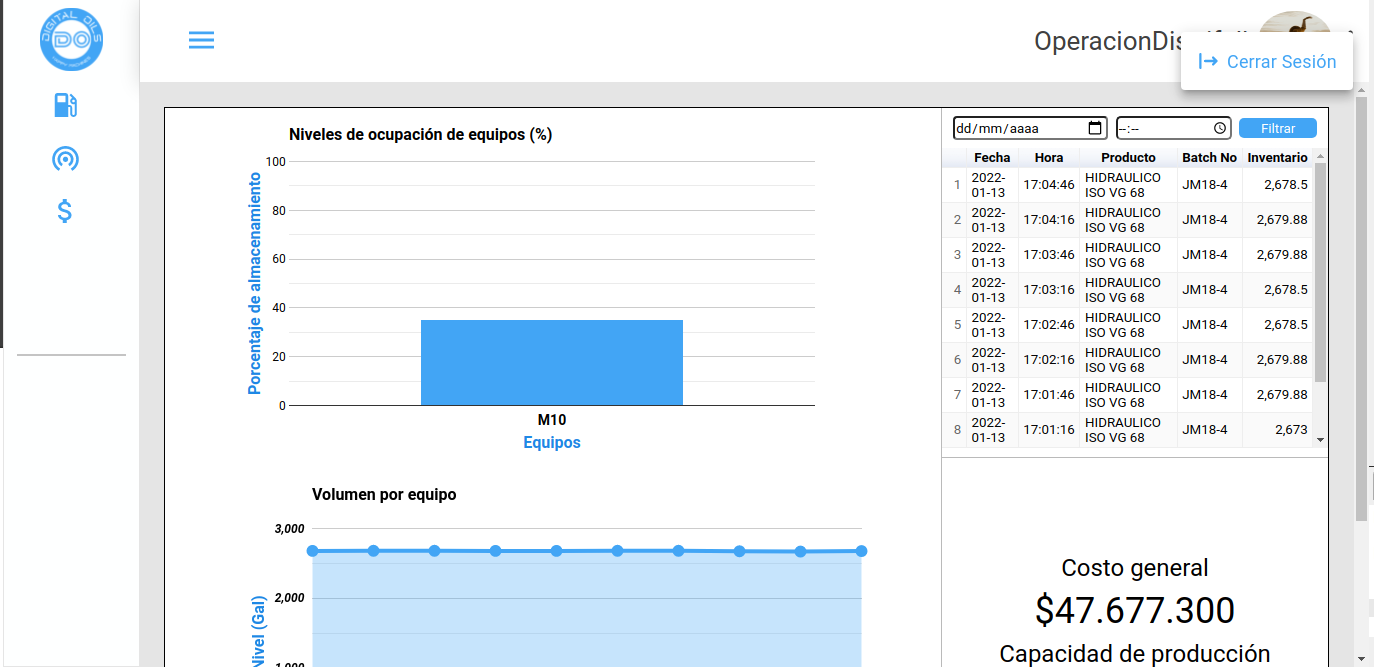
\includegraphics[width=1\linewidth, height=0.3\textheight]{imagenes/cerrarSesion}
	\caption[Cerrar sesi\'on.]{Cerrar sesi\'on}
	\label{fig:cerarsesion}
\end{figure}

Para cerrar sesi\'on presionamos en el bot\'on que tiene el aspecto de tres puntos verticales, ubicado al lado del avatar del usuario, una vez lo presionamos nos aparece la opci\'on de \textcolor{bluedistri}{cerrar sesi\'on}, seleccionamos esta opci\'on y esto finaliza la sesi\'on y nos redirige a la p\'agina principal.
\newpage
\subsection{Cambio de idioma}

\begin{figure}[h!]
	\centering
	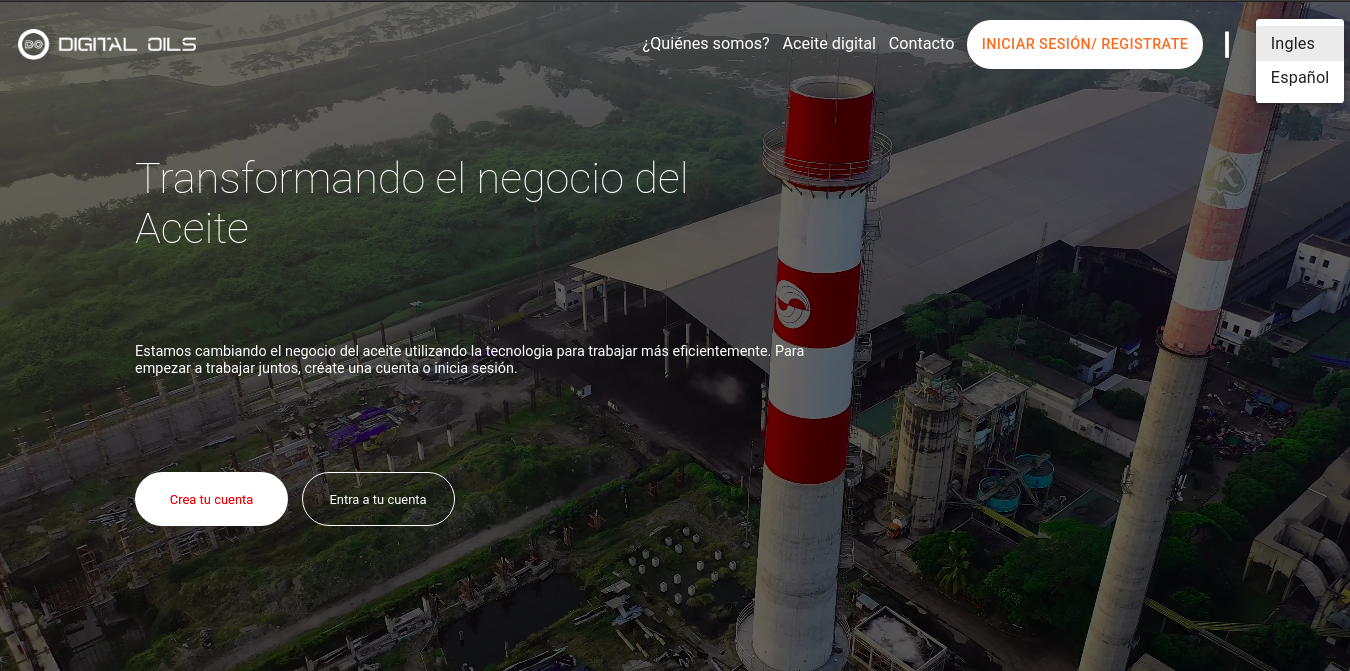
\includegraphics[width=1\linewidth, height=0.3\textheight]{imagenes/inicioOneIdioma}
	\caption[\'Area principal.]{}
	\label{fig:iniciooneidioma}
\end{figure}

El aplicativo web de Distrifull cuenta con dos idiomas, espa\~nol e ingl\'es, para cambiar el idioma de la plataforma seleccionamos el bot\'on {\bf espa\~nol} y nos aparecen las opciones para elegir el idioma, una vez seleccionemos una opci\'on, el cambio de idioma se realiza instant\'aneamente.
